\documentclass{article}
\usepackage{ijcai17}
\usepackage{times}
%Preamble File for Tutorial

\usepackage{times}
\usepackage{graphicx}
\graphicspath{{../../}{figures/}}
%Theorems and such

%\usepackage{amsthm}

\newtheorem{theorem}{Theorem}
%\newtheorem{observation}{Observation}
\newtheorem{proposition}{Proposition}
\newtheorem{definition}{Definition}

%\usepackage{proceed2e}
%\usepackage{ltexpprt}
% defines theorem environments etc.


%\newtheorem{theorem}{Theorem}[section]
\newtheorem{observation}{Observation}[section]
\newtheorem{hypo}{Hypotheses}[section]
%\newtheorem{proposition}{Proposition}[section]
%\newtheorem{definition}{Definition}[section]

%%%%%%%%%%%%%%%%%%
% Packages
%%%%%%%%%%%%%%%%%%

\usepackage[ruled,vlined]{algorithm2e}
\usepackage{algorithmic}
%\usepackage{amsthm}
\usepackage{amsmath}
\usepackage{amsfonts}
\usepackage{amssymb}
\usepackage{graphicx}
\usepackage{url}
\usepackage{subfigure}
\usepackage{epstopdf}
%\setcounter{MaxMatrixCols}{30}
\usepackage{multirow}
\usepackage{subfigure}
\usepackage{ifthen}
\DeclareMathOperator*{\argmax}{argmax}
\DeclareMathOperator*{\argmin}{argmin}
\DeclareMathOperator{\NP}{\mathbf{\mathrm{NP}}}

%%%%%%%%%%%%%%%%%%%%
% font styles
%%%%%%%%%%%%%%%%%%

\def\defterm#1{\textbf{#1}}
%\def\set#1{\mathbf{#1}}
\def\set#1{\bs{#1}}
\def\bs#1{\boldsymbol{#1}}
\def\ground#1{\overline{#1}}


%%%%%%%
% values
%%%%%%%

\newcommand{\male}{M}
%%%%%%%%
% other systems

\newcommand{\foil}{\textsc{FOIL}}
%%%%%%%%%%%%%%%%%%%
% relational structures
%%%%%%%%%%%%%%%%%%

\newcommand{\structure}{w}
\newcommand{\individuals}{\mathcal{I}}
\newcommand{\functors}{\mathcal{F}}\newcommand{\values}{\mathcal{V}}
\newcommand{\samplesize}{N}
\newcommand{\psize}[2]{N\left[#1;#2\right]}
%usage{\psize{population}{dstructure}
\newcommand{\varsize}[2]{\psize{#1}{#2}}
%usage \varsize{pvariable}{dstructure}
%%%%%%%%%
% special functors


% for population variables
\newcommand{\Avariable}{\mathbb{A}}
\newcommand{\Bvariable}{\mathbb{B}}
\newcommand{\Cvariable}{\mathbb{C}}
\newcommand{\Uvariable}{\mathbb{U}}

%for individual constants
\newcommand{\aconstant}{a}
\newcommand{\bconstant}{b}
\newcommand{\cconstant}{c}

% for classes, sorts, types

\def\varclass#1#2{#1_{#2}}
%usage \varclass{\individuals}{\Avariable}


% for functors

\newcommand{\functor}{f}
\newcommand{\Ppredicate}{P}
\newcommand{\Rpredicate}{R}
\newcommand{\class}{\it{Class}}
% for functors representing classes
\newcommand{\indclass}{\individuals}
\newcommand{\relationship}{\it{Relation}}
% for functors representing classes

% various constants
\newcommand{\true}{\mathrm{T}}
\newcommand{\false}{\mathrm{F}}
\newcommand{\na}{\it{na}}
\newcommand{\normalconstant}{Z} % the normalization constant

%formulas and such
%first-order variables
\newcommand{\Xvariable}{X}
\newcommand{\Yvariable}{Y}
\newcommand{\numvalues}[1]{r_{#1}}
% usage \numvalues{i}
%terms and compounds
\newcommand{\term}{\tau}
\def\fterm#1#2{#1(#2)}
%usage \term{\functor}{\terms}
\newcommand{\literal}{l}
\newcommand{\conjunction}{C}
\newcommand{\formula}{\phi}
\newcommand{\numformulas}{m}

%%%%%%%%%%%%%%%%%%
% Groundings
%%%%%%%%%%%%%%
\def\FG#1{#1^{\ast}}
\newcommand{\grounding}{\gamma}
\def\groundnode#1{\gamma_{#1}}
\def\replace#1#2{#1\backslash#2}
% \replace{population variable \textbackslash constant
\def\ground#1#2{\FG{#1}_{#2}}
%usage: \groundobject{object}{grounding}
\def\instantiate#1#2{#1_{#2}}
\def\groundall#1{\Gamma_{#1}}
% \groundall{Gamma}{set of pvariables}
%the substitution space of a set of variables

\def\resultset#1#2{\mathcal{R}_{#1}(#2)}
%usage \resultset{structure}{formula}

% Annotations marking degree of grounding
\newcommand{\UG}[2][0.0ex]{#2^{-}\hspace{#1}}
\newcommand{\PG}[2][0.0ex]{#2^{\prime}\hspace{#1}}
%\newcommand{\FG}[2][0.0ex]{#2^{*}\hspace{#1}}


%%%%%%%%%%%%%%%%
% Counts and probabilities
%%%%%%%%%%%%%%%%

\newcommand{\dset}{D}
\newcommand{\dstructure}{\mathcal{D}}
% observed substructure
\def\dminus#1#2{\FG{#1}_{-#2}}
%usage: \dminus{dstructure}{ground atom}
%\def\dvalues#1#2#3{#1_{#2}(#3)}
%%observed values in D. usage: dvalues{values}{variables}{Database}
\def\dvalues#1#2#3{#1^{#2}_{#3}}
%observed values in D. usage: dvalues{varvalue}{grounding}{Database}
\def\dprob#1#2{P_{#1}(#2)}

%%%%%%%%%
% deprecate these
\def\dlog#1#2{L_{#1}(#2)}
% usage: dprob{structure}{formula}
\def\dlogcount#1#2#3{L^{#1}_{#2}(#3)}
% usage: L{model}{node index}{database}
\def\dlogfreq#1#2#3{\nscore{L}^{#1}_{#2}(#3)}
% usage: L{model}{node index}{database}
\def\aiclocal#1#2#3{\it{AIC}^{#1}_{#2}(#3)}
% usage: AIC{model}{node index}{database}
\def\aicfreq#1#2#3{\nscore{\it{AIC}}^{#1}_{#2}(#3)}
% usage: AIC{model}{node index}{database}
\def\biclocal#1#2#3{\it{BIC}^{#1}_{#2}(#3)}
% usage: BIC{model}{node index}{database}


\def\spenalty#1#2#3#4{f^{#1}(\numpars{#3}{#2},#4)}
%usage \spenalty{scorename}{node index}{graph}{countvector}

\def\numpars#1#2{\#\it{pars}_{#2}(#1)}
% usage \numpars{\BN}{i}

\def\Score#1#2#3{#1(#2,#3)}
%usage \Score{scorename}{\BN}{\D}
\def\score#1#2#3#4{#1_{#2}(#3,#4)}
%\def\score#1#2#3#4{#1_{#3}(#2,#4)}
% usage: \score{scorename}{node index}{graph}{database}
% usage: \score{scorename}{node index}{parents}{database}
%\def\gain#1#2#3#4#5{\improve{#1}_{#4}(#2,#3',#5)}
\def\Gain#1#2#3#4{#1(#2,#3,#4)}
%usage \Gain{gainname}{\BN}{\BN'}{dstructure}
\def\gain#1#2#3#4{#1_{#2}(#3,#3^{+},#4)}
% usage: \gain{scorename}{node index}{model}{database}
\newcommand\parloss[2]{\improve{\it{pars}}({\node_{i},{\Parents{#1}{#2},\node_{+}}})}
%usage: parloss{node index}{model}
%score names


\newcommand{\loglikelihood}{LL}
\newcommand{\aic}{AIC}
\newcommand{\bic}{BIC}
\newcommand{\bdeu}{BDeu}
\newcommand{\rescale}{\loglikelihood_{\it{scale}}}

\def\cscore#1{#1}
%count score
\def\nscore#1{\overline{#1}}
%\def\nscore#1{#1}
% normalized score
\def\ncscore#1{\widetilde{#1}}
%\def\gain#1{\overline{#1}}
\def\improve#1{\Delta#1}
\def\logimprove#1#2#3#4{\improve{L}^{#1,#2}_{#3}(#4)}
%usage \logimprove{BN1}{BN2}{i}{dstructure}
\def\flogimprove#1#2#3#4{\improve{\nscore{L}}^{#1,#2}_{#3}(#4)}
%usage \logimprove{BN1}{BN2}{i}{dstructure}
\def\aicimprove#1#2#3#4{\improve{\nscore{\it{AIC}}}^{#1,#2}_{#3}(#4)}
\def\bicimprove#1#2#3#4{\improve{\nscore{\it{BIC}}}^{#1,#2}_{#3}(#4)}

\def\rlog#1#2{\Relevant{L}_{#1}(#2)}
\def\bprob#1#2#3{#1_{#2}(#3)}
% usage: bprob{P}{BN}{assignment}
\def\iprob#1{\FG{P}(#1)}
% usage iprob{ground formula/term}
\newcommand{\probworlds}{\mu}
%distribution over structures


%%%%%%%%%%%%
%DB counts
%%%%%%%%%

\newcommand{\Cvar}{\mathrm{n}}
\newcommand{\Fvar}{\mathrm{p}}
\newcommand{\Relevant}[1]{#1^{\mathrm{r}}}
\newcommand{\relevant}[1]{\it{R}_{#1}}
%usage \relevant{index}

\newcommand{\Count}[2]{\Cvar\left[#1;#2\right]}
%e.g.n[formula;database]
\newcommand{\Fcount}[3]{\Cvar^{#1}_{#2}(#3)}
%usage \fcount{\bn}{ijk}{dstructure}
\newcommand{\Fbcount}[3]{\set{\Cvar}^{#1}_{#2}(#3)}
\newcommand{\Fpcount}[3]{\overline{\set{\Cvar}}^{#1}_{#2}(#3)}
\newcommand{\Rcount}[3]{\Relevant{\Cvar}\left[{#1};#2\right]}
%usage \Rcount{formula}{dstructure}
\newcommand{\Frcount}[3]{\Relevant{\Cvar}_{#1}(#2)}
%usage \Rcount{ijk}{dstructure}
\newcommand{\countvec}[3]{\set{\Cvar}^{#1}_{#2}(#3)}
%usage \countvec{countvector symbol}{graph}{data}


\newcommand{\Freq}[2]{\Fvar\left[#1;#2\right]}
%e.g.n[formula;database]
\newcommand{\Ffreq}[2]{\Fvar_{#1}(#2)}
%usage \ffreq{ijk}{dstructure}
\newcommand{\Rfreq}[2]{\Relevant{\Fvar}\left[{#1};#2\right]}
%usage \Rfreq{formula}{dstructure}
\newcommand{\Frfreq}[2]{\Relevant{\Fvar}_{#1}(#2)}
%usage \Rfreq{ijk}{partial grounding}{dstructure}


%\newcommand{\Freq}[2]{\Fvar\left[#1;#2\right]}
%%e.g.n[formula;database]
%\newcommand{\Rfreq}[2]{\Relevant{\Fvar}\left[#1;#2\right]}
%\newcommand{\Ffreq}[2]{\Fvar_{#1}(#2)}
%%usage \fcount{ijk}{dstructure}
%\newcommand{\Frfreq}[2]{\Relevant{\Fvar}_{#1}(#2)}

%


%\newcommand{\Count}[2]{#1(#2)}
%%count of database
%%usage \bncount{\Cvar_{ijk}}{dstructure}
%\newcommand{\CountC}[2]{\Cvar_{ijk}\left[#1;#2\right]} %count in database satisfying grounding

%\newcommand{\drcount}[1]{\Relevant{\Cvar}_{ijk}\left[#1\right]}
%%count of database
%\newcommand{\drcountC}[2]{\Relevant{\Cvar}_{ijk}\left[#1;#2\right]} %count in database satisfying grounding
%
%\newcommand{\dfreq}[2]{#1(#2)}
%%frequency database
%\newcommand{\dfreqC}[2]{\Fvar_{ijk}\left[#1;#2\right]} %frequency in database satisfying grounding
%\newcommand{\drfreq}[1]{\Relevant{\Fvar}_{ijk}\left[#1\right]}
%%frequency in database
%\newcommand{\drfreqC}[2]{\Relevant{\Fvar}_{ijk}\left[#1;#2\right]} %frequency in database satisfying grounding



%%%%%%%%%%%%%%%%%%%%%%
% Bayesian networks
%%%%%%%%%%%%%%%%



% Functions for graph structure
\newcommand{\BN}{B}
\newcommand{\mln}{M}
\newcommand{\node}{\Xvariable}
\newcommand{\graph}{G}
\newcommand{\MB}[1]{\mathrm{MB}(#1)}
\newcommand{\bnparents}{\mathrm{Pa}}
\newcommand{\Parents}[2]{\mathrm{Pa}_{#1}^{#2}}
%usage \Parents{\nodeindex}{\model}
\newcommand{\pavalue}[2]{\mathbf{pa}_{#1}^{#2}}
%usage \pavalue{i}
\newcommand{\numparents}[2]{q_{#1}^{#2}}
% usage \numparents{i}{\graph}
\def\numpars#1#2{\#\it{pars}_{#2}^{#1}}
% usage \numpars{\BN}{i}
\newcommand{\Ch}[1]{\mathrm{Ch}(#1)}
\newcommand{\nodevalue}{\it{v}}
\newcommand{\xvalue}{x}
\newcommand{\yvalue}{y}
%\newcommand{\parent}{\mathit{pa}}


\newcommand{\parameter}{\theta}
% Key functions for parameters
\newcommand{\w}{w}
\newcommand{\mprob}[2]{#1(#2)}
% usage \mprob{P}{node_{i = value k}}
%marginal probability
\newcommand{\cprob}[3]{#1(#2|#3)}
%usage \cprob{P}{x}{y}
\newcommand{\estcprob}[1]{\widehat{\parameter}_{ijk}(#1)}
%usage \estcprob(\dstructure)


\newcommand{\family}[2]{#1^{#2}}
%usage: \family{\node}{i}
\newcommand{\familyvalue}[1]{\xvalue_{#1}}
%usage: \familyvalue{ijk}
\newcommand{\familyf}[2]{(\node_{#1},\Parents{\node_{#1}})=\xvalue_{#2}}
%% usage: \familyf{i}{ijk}

%%%%%%%%%%%%%%
%
% conditional probabilities in log-linear model

\newcommand{\Gpvar}{\FG{P}}
\newcommand{\Gprob}[2]{\Gpvar(#1 | #2)}







\usepackage{amssymb}
\usepackage{graphicx}
\usepackage[small]{caption}
%\usepackage{subcaption}
\usepackage{url}

\title{Model Selection Scores for Multi-Relational Bayesian Networks\thanks{Supported by a Discovery Grant from the Natural Sciences and Engineering Research Council of Canada.}\\
Extended Abstract for DeLBP Workshop at IJCAI 2017}

\author{Sajjad Gholami, Oliver Schulte, Vidhi Jian, Qiang Zhao\\ 
School of Computing Science\\
Simon Fraser University, Burnaby, Canada\\
\{oschulte,sgholami\}@cs.sfu.ca}

\begin{document}
\maketitle  
\begin{abstract} Many organizations maintain their data in a relational database, which contains information about entities, their attributes, relationships among the entities, and attributes of the relationships. Statistical-relational learning (SRL)
aims to generalize traditional single-table machine learning methods for multi-relational data. Many SRL models are defined using a combination of graphs and first-order logic.  This lecture addresses the task of learning the graph structure of a first-order Bayesian network (BN). A key component of structure learning is a model selection score that measures how well a model fits a dataset. We introduce a new method that generalizes for multi-relational databases, a BN score designed for single-table data.
%A multi-relational statistical model provides an integrated analysis of the interdependent and interdependent data resources in the database. 
We present several applications that leverage a learned model, such as modeling database statistics, exception mining, and extracting features for classification and anomaly detection. 
% Our main theorem provides an asymptotic statistical consistency guarantee for the method. Empirical evaluation on six benchmark relational databases shows that our relational model selection criterion is also practically useful: On realistic size data sets, it selects informative BN structures  with a better data fit than those selected by baseline model selection scores.
%{\bf keywords: } Model Selection, Statistical-Relational Learning, Bayesian Networks
\end{abstract}

\section{Introduction: Relational Learning}
%Relational data provide information about entities, their attributes, relationships among the entities and attributes of the relationships. 
Multi-relational databases in SQL format are very widely used to store enterprise data. Relational data are also known as network data, graph data, matrix data, and tensor data. Traditional machine learning analyzes  data represented in a single table; such data can be viewed as a special limiting case of multi-relational data with no relationships \cite{Nickel2016}. The field of statistical-relational learning (SRL)
aims to generalize single-table machine learning methods for multi-relational data; this is called {\em upgrading} the method~\cite{SRL2007,Ch.10deraedt}. Application domains for statistical-relational models include natural language processing, 
ontology matching, information extraction, entity resolution, link-based clustering, query optimization, representing uncertainty in databases, etc 
\cite{Domingos2007,Niu2011,Getoor2001,Wang2008}. This lecture addresses the important SRL task of learning the structure of a first-order Bayesian  structure from a relational dataset. Our presentation describes several applications that leverage a learned model, such as modeling database statistics, exception mining, and extracting features for classification and anomaly detection. 

 
The most common approach to BN structure learning is to search for a structure that maximizes a model selection score for a given dataset. Our companion paper \cite{Schulte2017a} introduces a general method for upgrading BN model selection scores. 
%
This outline illustrates the method for the case of likelihood-based scores, which take the form (log-likelihood of data under model) - penalty(model, sample size, \#number parameters). %Example scores include  \aic~ and \bic. 
The full paper defines the method for BN scores in general, with more examples and references.

\section{Background and Notation} 
We assume familarity with basic BN concepts such as DAGs and conditional probability tables.
We adopt  
a function-based  formalism for combining relational and statistical concepts~\cite{Poole2003,Russell2015}. For a set of random variables $\set{\node} = \{\node_{1},\ldots,\node_{n}\}$, 
%The possible values of $\node_{i}$ are enumerated as $\{\xvalue_{i1},\ldots,\xvalue_{i\states_{i}}\}$. 
%The notation $P(\node_{i} = \xvalue)\equiv P(\xvalue)$ denotes the probability of random variable $\node_{i}$ taking on value $\xvalue$. 
%We also use 
the  notation $P(\set{\node} = \set{\xvalue}) \equiv P(\set{\xvalue})$ denotes the joint probability that each random variable $\node_{i}$ takes on value $\set{\xvalue}_{i}$. 

\paragraph{Relational Data} 

A multi-relational model is typically a multi-population model. A \textbf{population} is a set of individuals of the same type (e.g., a set of $\it{Users}$, a set of $\it{Movies}$). Individuals are 
denoted by %lower-case 
constants (e.g., $\it{user}_{3}$,$\it{thor}$). 
%
A $k$-ary \textbf{functor}, denoted $\functor,\functor'$ etc.,  maps a tuple of $k$ individuals to a value from the functor's \textbf{domain}. The arguments of a functor are restricted to appropriate types. Throughout the paper we assume complete data. A complete relational \defterm{database} $\dstructure$ specifies:

\begin{enumerate}
\item A finite sample population $\individuals_{1},\individuals_{2}\ldots$, one for each type. 
%Each sample size is denoted by $\psize{\individuals_{i}}{\dstructure}$.
\item The values of each functor, for each input tuple of observed sample individuals of the appropriate type.
\end{enumerate}

Figure~\ref{fig:database} shows a toy database. The example follows the closed-world convention: if a relationship between two individuals is not listed, it does not obtain.

\begin{figure}[tb]
	\centering
	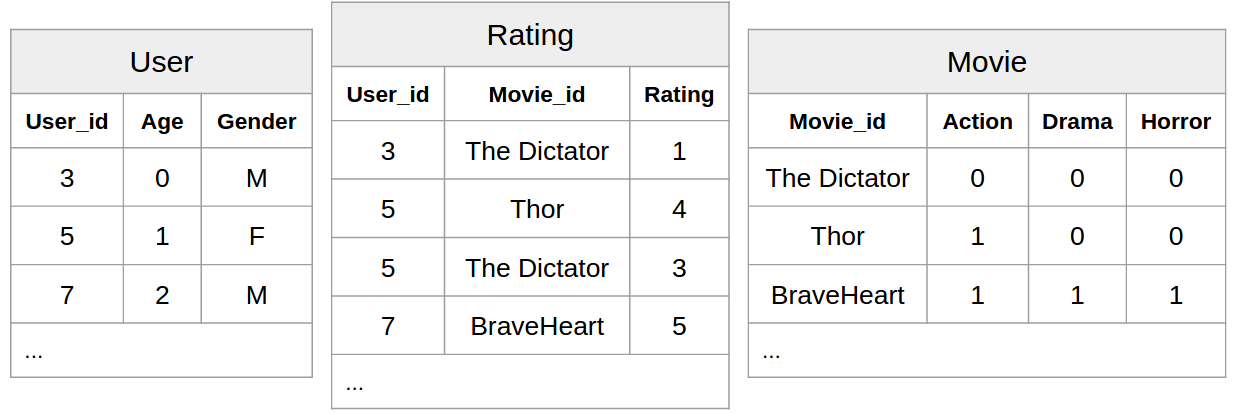
\includegraphics[width=0.48\textwidth] 
	{relExample}
	\caption{Excerpt from a relational dataset/database.} 
	\label{fig:database}
\end{figure}

\paragraph{Relational Random Variables} 


A \textbf{population}  variable ranges over a population, and is denoted in upper case such as $\it{User},\it{Movie}, \Avariable$.
%,\Bvariable$. A %(functional) 
A \textbf{term} is of the form $f(\term_{1},\ldots,\term_{k})$ where each $\term_{i}$ is a population variable or a constant/individual of the appropriate type.  A first-order random variable (FORV) is a term with at least one population variable~\cite{Wang2008}. A first-order Bayesian network (FOB)~\cite{Wang2008}, aka Parametrized BN~\cite{Kimmig2014}, is a BN whose nodes are FORVs.  Figure~\ref{fig:bn} shows two FOBs. The rating value is n/a (for ``not applicable'') if and only if the user has not rated the movie (cf.~\cite{Russell2010}). Throughout the paper, conditional probability estimates are computed from the IMDb database.

\begin{figure}[tb]
	\centering
	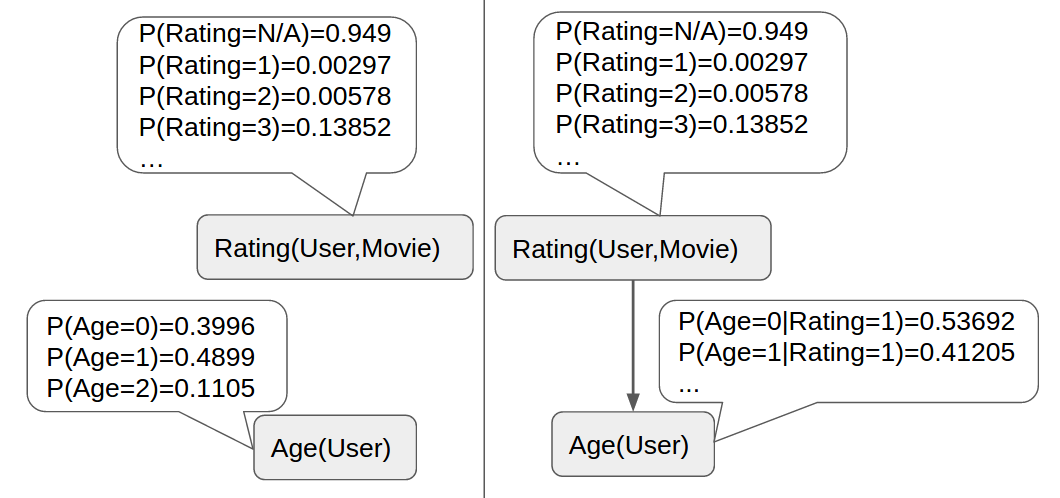
\includegraphics[width=0.48\textwidth] 
	{bnstructIjcai}
	\caption{Example First-Order Bayesian networks: left = $\BN_{1}$  with graph $\graph_{1}$, right = $\BN_{1}^+$ with graph $\graph_{1}^+$. %The type of population variables is shown as in a plate model. 
		\label{fig:bn}}
\end{figure}

The \defterm{database frequency} \cite{Halpern90} of an assignment $\set{\Xvariable} = \set{\xvalue}$ is the number of satisfying groundings over the number of possible groundings: 

\begin{equation} \label{eq:proportion}
\dprob{\dstructure}{\set{\Xvariable} = \set{\xvalue}} 
= \frac
{\Count{\set{\Xvariable} = \set{\xvalue}}{\dstructure}}
{\psize{\set{\Xvariable} = \set{\xvalue}}{\dstructure}
}
\end{equation}
where $\Count{\set{\Xvariable} = \set{\xvalue}}{\dstructure}$ denotes the \defterm{number of satisfying groundings} that satisfy the assignment in database $\dstructure$, and  $\psize{\set{\Xvariable} = \set{\xvalue}}{\dstructure}$ denotes the total number of possible groundings of the variables in the list  $\set{\Xvariable}$.


Using the standard BN product formula, a FOB $\BN$ represents a joint distribution over assignments to first-order random variables, written $\bprob{P}{\BN}{\set{\node} = \set{\xvalue}}$. A model selection score measures how well the model distribution $P_\BN$ fits the empirical or \emph{database distribution} $\dprob{\dstructure}{\set{\Xvariable} = \set{\xvalue}}$.
%, which is defined as follows~\cite{Halpern90,Schulte2014}.  The \defterm{number of possible groundings} of a joint assignment is given by $\psize{\set{\Xvariable} = \set{\xvalue}}{\dstructure} \equiv \varsize{\Avariable_{1}}{\dstructure} \times \cdots \times \varsize{\Avariable_{m}}{\dstructure}$ where the $\Avariable_{i}$ are the population variables in $\set{\Xvariable}$ and $\varsize{\Avariable}{\dstructure}$ is the size of the sample population of $\Avariable$.
%The \defterm{number of satisfying groundings} of a joint assignment in database $\dstructure$ is denoted by 
%$\Count{\set{\Xvariable} = \set{\xvalue}}{\dstructure}$. The \defterm{database frequency} \cite{Halpern90} is the number of satisfying groundings over the number of possible groundings: 
%
%\begin{equation} \label{eq:proportion}
%\dprob{\dstructure}{\set{\Xvariable} = \set{\xvalue}} 
%= \frac
%{\Count{\set{\Xvariable} = \set{\xvalue}}{\dstructure}}
%{\psize{\set{\Xvariable} = \set{\xvalue}}{\dstructure}
%}.
%\end{equation}
%
Table~\ref{table:frequency} compares database frequencies using the IMDb dataset to BN model probabilities. The expanded BN $\BN_{1}^+$ matches the database distribution perfectly but at the cost of more parameters. 

\begin{table}[tb]
\caption{The IMDb database frequency of a joint assignment to first-order random variables, compared to the BN probabilities computed using the network parameters of Figure~\ref{fig:bn}.}
\begin{center}
\resizebox{0.5\textwidth}{!}{
\begin{tabular}{|r|r|r|}
\hline
$\set{\Xvariable}=\set{\xvalue}$ & \begin{tabular}{l}$\it{Age(User)=0}$\end{tabular} & \begin{tabular}{l}$\it{Age(User)=0},$\\ $\it{Rating(User,Movie)=1}$\end{tabular}  \\\hline
$\Count{\set{\Xvariable} = \set{\xvalue}}{\dstructure}$ & 376 & 2,524 \\\hline
$\psize{\set{\Xvariable} = \set{\xvalue}}{\dstructure}$ & 941 & 1,582,762  \\\hline 
$\dprob{\dstructure}{\set{\Xvariable} = \set{\xvalue}} $ & $376/941 \approx 0.3996$ & $2,524/1,582,762 \approx 0.0016$ \\\hline
$\bprob{P}{\BN_1}{\set{\node} = \set{\xvalue}}$ & 0.3996 & $0.00297 \cdot 0.3996 \approx 0.0012$ \\\hline
$\bprob{P}{\BN_{1}^+}{\set{\node} = \set{\xvalue}}$ & 0.3996 & $0.00297 \cdot 0.53692 \approx 0.0016$ \\\hline
\end{tabular}
}
\end{center}
\label{table:frequency}
\end{table}%


\section{Relational Likelihood Score}
A fundamental model score is the class likelihood function, which measures how likely the data is given the model.
In previous work on parameter learning, \cite{Xiang2011,Schulte2011}, the log-likelihood score $\loglikelihood$ for i.i.d. data was upgraded by the \defterm{normalized log-likelihood score} NLL. The NLL score can be computed in closed-form given the BN \defterm{sufficient statistics}, which we denote as follows. Let $\node_{i} = \xvalue_{ik},\Parents{i}{\graph}=\pavalue{ij}{\graph}$ be the assignment that sets node $i$ to its $k$-th value, and its parents to their $j$-th possible configuration. 

\begin{itemize}
\item $\Fcount{G}{ijk}{\dstructure} \equiv \Count{\node_{i} = \xvalue_{ik},\Parents{i}{G}=\pavalue{ij}{G}}{\dstructure}$ is the number of groundings that satisfy the $ijk$ assignment.
\item $\Fcount{G}{ij}{\dstructure} \equiv \sum_{k} \Fcount{G}{ijk}{\dstructure}$ is the number of groundings that satisfy the $j$-th parent assignment.
\item $\Fcount{G}{i}{\dstructure} \equiv \sum_{j}\sum_{k} \Fcount{G}{ijk}{\dstructure}$ is the number of possible groundings for node $i$, called the \defterm{local sample size}.
\end{itemize}

In relational sufficient statistics {\em the local sample size  $\Fcount{G}{i}{\dstructure}$ depends on the graph structure} whereas in i.i.d. data, the number of data points defines a global sample size that is the same for all nodes and all graph structures. The NLL score is defined as
$$
 \score{\nscore{\loglikelihood}}{i}{G}
 {\dstructure}
  \equiv  \sum_{i} \frac{1}{\Fcount{G}{i}{\dstructure}}\sum_{j} \sum_{k} \Fcount{\graph}{ijk}{\dstructure} \cdot 
\log_{2} \left(\frac
{\Fcount{\graph}{ijk}{\dstructure}}{\Fcount{\graph}{ij}{\dstructure}}\right)
$$

The normalization $1/\Fcount{G}{i}{\dstructure}$ converts different sufficient statistics to proportions and therefore the same [0,1] scale. 
Table~\ref{table:likelihood-example} illustrates the importance of re-scaling counts. The $\score{\loglikelihood}{i}{\cdot}{\Fbcount{\cdot}{ijk}{\cdot}}$ column shows the likelihood score with instantiation counts. This term is an order of magnitude lower for the expanded BN structure $G_{1}^+$ (-2266 vs. -497),  simply because the expanded structure increases the local sample size by the number of Movies. 


\begin{table*}[tb]\centering
\resizebox{0.9\textwidth}{!}{
\begin{tabular}{|l|r|l|r|r|r|r|r|}
\hline
Family Configuration & \multicolumn{1}{l|}{$n_{ijk}$} & $n_{ij}$ & \multicolumn{1}{l|}{$n_{i}$} & \multicolumn{1}{l|}{$n_{ijk}/n_i$} & \multicolumn{1}{l|}{\emph{CP}} & \multicolumn{1}{l|}{$\score{\loglikelihood}{i}{\cdot}{\Fbcount{\cdot}{ijk}{\dstructure}}$} & \multicolumn{1}{l|}{$\frac{\score{\loglikelihood}{i}{\cdot}{\Fbcount{\cdot}{ijk}{\dstructure}}}{\Fcount{G^{+}}{i}{\dstructure}}
$} \\ \hline
\begin{tabular}{l}Age(User)=0\end{tabular} & 376 & --- & 941 & 0.3996 & 0.3996 & -497.6217 & -0.5288 \\ \hline
\begin{tabular}{l}Age(User)=0, \\Rating(User,Movie)=1\end{tabular} & 2524 & \multicolumn{1}{r|}{4703} & 1582762 & 0.0016 & 0.5367 & -2266.2224 & -0.0014 \\ \hline
\end{tabular}
}
\caption{For the node $\it{Age(User)}$, and the IMDb dataset, the contribution of one family configuration to the unnormalized resp. normalized log-likelihood score. Top: For the $G_{1}$ structure of Figure~\ref{fig:bn}. Bottom: For the expanded structure $G_{1}^+$.
\label{table:likelihood-example}}
\end{table*}


\section{Relational Likelihood-Based Scores}

In i.i.d. data, a likelihood-based score $S$ subtracts a model complexity term from the log-likelihood score. We subtract a model complexity term from the NLL score to compare two BN structures $\graph$ and $\graph^{+}$. Assuming that $\graph^{+}$ adds edges to $\graph$, our method is to compute, the improvement or \defterm{normalized gain} of $\graph^{+}$ over $\graph$ as follows: 

\begin{equation}\label{eq:nll-diff}
[\score{\nscore{\loglikelihood}}{i}{\graph^{+}}{ {\dstructure}}-\frac{f_{i}(\graph^{+})}{\Fcount{\graph^{+}}{i}{\dstructure}}] - [\score{\nscore{\loglikelihood}}{i}{\graph}{\dstructure}-\frac{f_{i}(\graph)}{\Fcount{\graph^{+}}{i}{\dstructure}}]
\end{equation}

where for the smaller BN $\BN$, the local complexity $f_{i}(\BN)$ is computed 
using the sample size for the {\em larger}  structure. Normalizing {\em both} penalty terms by the same sample size measures them on the same scale. 
Table~\ref{table:comparison-scores} gives the formulas for the $\aic$ and $\bic$  penalty terms. 
%For such likelihood-based scores, our single-model score upgrade methods add a penalty term to the normalized log-likelihood. 
Table~\ref{table:compute-scores} shows example values for the gains. 

Since the normalized gain term for the smaller structure $\graph$ depends on the sufficient statistics for the comparison structure $\graph^{+}$, {\em the normalized gain cannot be represented as the differential of two single-model scores.} Our baseline single-model scores extend the normalized log-likelihood score $\nscore{\loglikelihood}$ %established in previous work 
with a penalty term. The \defterm{count method} simply adds the penalty term $f_{i}(\graph)$; the \defterm{normalized method} divides the penalty term by the local sample size (i.e., $f_{i}(\graph)/\Fcount{\graph}{i}{\dstructure}$).

%\begin{table}[tbhp]
%\resizebox{0.5\textwidth}{!}{
%\begin{tabular}{|  c | c |}
%     $\aic_{i}$ &$\aic_{i}$  \\\
%	\hline
%  Normalized Gain & $\frac{(\numpars{G^{+}}{i} - \numpars{G}{i})}{\Fcount{\graph^{+}}{i}{\dstructure}}$
% & $\frac{(\numpars{G^{+}}{i} - \numpars{G}{i}) \log_{2}(\Fcount{\graph^{+}}{i}{\dstructure})}{2 \Fcount{\graph^{+}}{i}{\dstructure}}$
% %\cdot \frac{\log_{2}(\Fcount{\graph^{+}}{i}{\dstructure})}{2 \Fcount{\graph^{+}}{i}{\dstructure}}$ \\
% \\\hline
%%Count Score 
%%& $ \numpars{G}{i}$
%%&$ \numpars{G}{i} \cdot \frac{1}{2}\log_2(\Fcount{G}{i}{\dstructure}) $
%%\\\hline
%% Normalized Score  & 
%%$ \frac{\numpars{G}{i}}{\Fcount{G}{i}{\dstructure}}$ &
%%$  \numpars{G}{i} \cdot \frac{\log_2(\Fcount{G}{i}{\dstructure}}{2 \Fcount{G}{i}{\dstructure}}$ \\\hline
%\end{tabular}
%} % end box
%\caption{Relational Penalty Terms for the $\aic$ and $\bic$ scores. 
%The normalized gain adds the penalty term to the normalized log-likelihood differential \eqref{eq:nll-diff}.}
%%defines the model selection criteria used in our experiments.} 
%\label{table:comparison-scores}
%\end{table}
%$\aic_{i}$ &$\aic_{i}$  \\\\hline

\begin{table}[tbhp]
\resizebox{0.5\textwidth}{!}{
\begin{tabular}{|  c | c |}
\hline
$\aic_{i}$ & $\bic_{i}$ \\ \hline
 $\frac{(\numpars{G^{+}}{i} - \numpars{G}{i})}{\Fcount{\graph^{+}}{i}{\dstructure}}$
 & $\frac{(\numpars{G^{+}}{i} - \numpars{G}{i}) \log_{2}(\Fcount{\graph^{+}}{i}{\dstructure})}{2 \Fcount{\graph^{+}}{i}{\dstructure}}$
 \\\hline
\end{tabular}
} % end box
\caption{Relational Local Penalty Terms for the $\aic$ and $\bic$ scores.  $\numpars{G^{+}}{i}$ is  the number of parameters for node $i$.
The normalized gain adds the penalty term to the normalized log-likelihood differential \eqref{eq:nll-diff}.}
\label{table:comparison-scores}
\end{table}

\begin{table*}[tbhp]\centering
\resizebox{0.9\textwidth}{!}{
\begin{tabular}{|l|c|c|c|c|c|c|c|c|c|}
\hline
 \multicolumn{1}{|l|}{} & \multicolumn{1}{l|}{} & \multicolumn{1}{l|}{} & \multicolumn{1}{c|}{} & \multicolumn{3}{c|}{AIC} & \multicolumn{3}{c|}{BIC}  \\ \hline
 & \multicolumn{1}{l|}{\#groundings} & \multicolumn{1}{l|}{\#parameters} & \multicolumn{1}{l|}{$\nscore{\loglikelihood}$} &  \multicolumn{1}{l|}{count} & \multicolumn{1}{l|}{normalized gain} & normalized & \multicolumn{1}{l|}{count} & \multicolumn{1}{l|}{normalized gain} & normalized \\ \hline
    $G_{1}$ & 941 & 2 & -1.384 &  -3.38 & ---  & -1.3865  & -11.26 & --- & -1.3948 \\%\hline
    $G_{1}^{+}$ & 1582762 & 12 & -1.177  & -13.18 & --- & -1.1775  & -124.74 & --- & -1.1776 \\ \hline
    GAIN &  & 10 & 0.207  & -9.79 & 0.20684 & 0.2090  & -113.48 & 0.20678 & 0.2173  \\\hline
\end{tabular}
}
\caption{Example values for the scores and gain functions defined in this section, for the IMDb dataset and the structures of Figure~\ref{fig:bn}. Note that count gain $<$ normalized gain $<$ normalized score gain. E.g., for $\aic$ gains  $ -9.79 < 0.020684  < 0.2090$.
\label{table:compute-scores}}
\end{table*}

\section{Theoretical Analysis}
We formalize consistency for relational data following previous work~\cite{Sakai2013,Xiang2011}. The notation $\set{\samplesize}(\dstructure) \rightarrow \infty$ from 
denotes that  each population size $\individuals_{i}$ goes to infinity. Chickering and Meek \citeyear{Chickering2002}
introduced the concept of  \defterm{local consistency}, which we adapt for  
gain functions. Let $p$ be the data generating distribution. A gain function is \defterm{locally consistent} if the following hold 
as $\set{\samplesize}(\dstructure) \rightarrow \infty$, for any graph $\graph$ and expansion $G_{+}$ that adds a single edge $\node_{+} \rightarrow \node_{i}$ to $\graph$: The gain of a DAG model is (1) positive for any edge that is necessary for representing the generative distribution $p$, and (2) is negative for any edge that is unnecessary. These clauses ensure statistical consistency---necessary edges are learned---and optimality---only necessary edges are learned~. A relational upgrade method \defterm{preserves local consistency} if local consistency for a single-table gain function entails local consistency for its upgrade.

%\begin{definition}
% Let $p$ be the data generating distribution. A gain function is \defterm{locally consistent} if the following hold 
% as $\set{\samplesize}(\dstructure) \rightarrow \infty$, for any graph $\graph$ and expansion $G_{+}$ that adds a single edge $\node_{+} \rightarrow \node_{i}$ to $\graph$:
%
%\begin{enumerate}
%\small
%\item If $\node_{+}$ is not independent of $\node_{i}$ given  $\Parents{i}{G}$ in $p$, then $\Gain{\Delta}{G}{G_{+}}{\dstructure} > 0$. \label{clause:consistency}
%\item If $\node_{+}$ is independent of $\node_{i}$ given  $\Parents{i}{G}$ in $p$, then $\Gain{\Delta}{G}{G_{+}}{\dstructure} < 0$. \label{clause:optimality}
%\end{enumerate}
%
%\end{definition}

%An upgrade method \defterm{preserves local consistency} if local consistency for an i.i.d. gain function entails local consistency for its upgrade. In the sample size limit, clause~\ref{clause:consistency} entails that 
%the gain of a DAG model is (1) positive for any edge that is necessary for eliminating an independence constraint that does not hold in the generative distribution, and (2) is negative for any edge that is unnecessary. Together, these clauses ensure consistency---necessary edges are learned---and optimality---only necessary edges are learned~\cite{Chickering2002}.

\begin{theorem} \label{th:consistency}
The normalized gain upgrade preserves local consistency, and therefore consistency. The single-model comparison scores do not preserve local consistency.
\end{theorem}

\section{Empirical Results}

We learn Bayesian network structures with the three model comparison criteria shown in Table~\ref{table:comparison-scores} on 6 benchmark datasets. The count score selects the {\em empty graph} on all. The normalized score selects graphs with many edges (almost complete). The normalized gain selects informative structures that strike a desirable balance between overly sparse and overly dense graphs.

\section{Conclusion} Generalizing single-table model scores for multi-relational data is an important fundamental topic for relational learning. The normalized gain, which measures the difference in data fit between two first-order Bayesian network structures, is a novel scalable method for generalizing a BN score. For complete data, it can be computed in closed form given the BN sufficient statistics. Normalized gain functions preserve convergence guarantees, and show good empirical performance: they select structures that succinctly represent the data correlations, compared with baseline single-model scores.
%
%A promising avenue for future work is to apply our approach to other statistical-relational models, such as Markov Logic Networks.

\bibliographystyle{named}
\bibliography{master}

\end{document}
\maketitle
